\subsection{Development Process}
The minimum viable artefact is a Python notebook file containing Python scripts to run the experiment.
We run the notebook with IBM Quantum Experience, as they provide online services for simulating quantum hardware.
The following sections describe our experiment process.

\subsubsection{The Quantum Emulator}
For this experiment, we are using the Quantum Emulator provided by Qiskit.
The QASM simulator is used to mimic an IBMQ device.
We don't configure the noise model for emulator. 
Additionally, QASM simulator by default has no noise, so we can expect the result to be noise-free.

\subsubsection{Creating Ansatzes}
We have chosen two ansatzes \textit{NLocal} and \textit{TwoLocal} from the Qiskit circuit library due to their wide usage in quantum machine learning.
As discussed in the Research Design section, we configure the ansatz objects such that their gradient variances decrease exponentially with the number of qubits.
These characteristics are:
\begin{itemize}
    \item The circuit depth;
    \item The number of qubits to be measured for the cost function;
    \item The randomised parameters.
\end{itemize}
An example of circuits generated by Qiskit is visualised in Figure \ref{Ansatz samples}.

\begin{figure}
    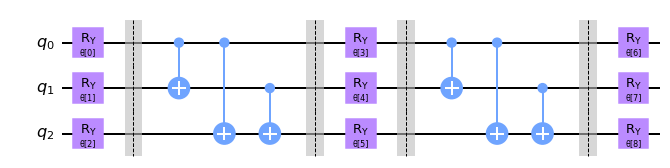
\includegraphics[width=\textwidth]{Artefact/Appendices/ansatz3-2.png}
    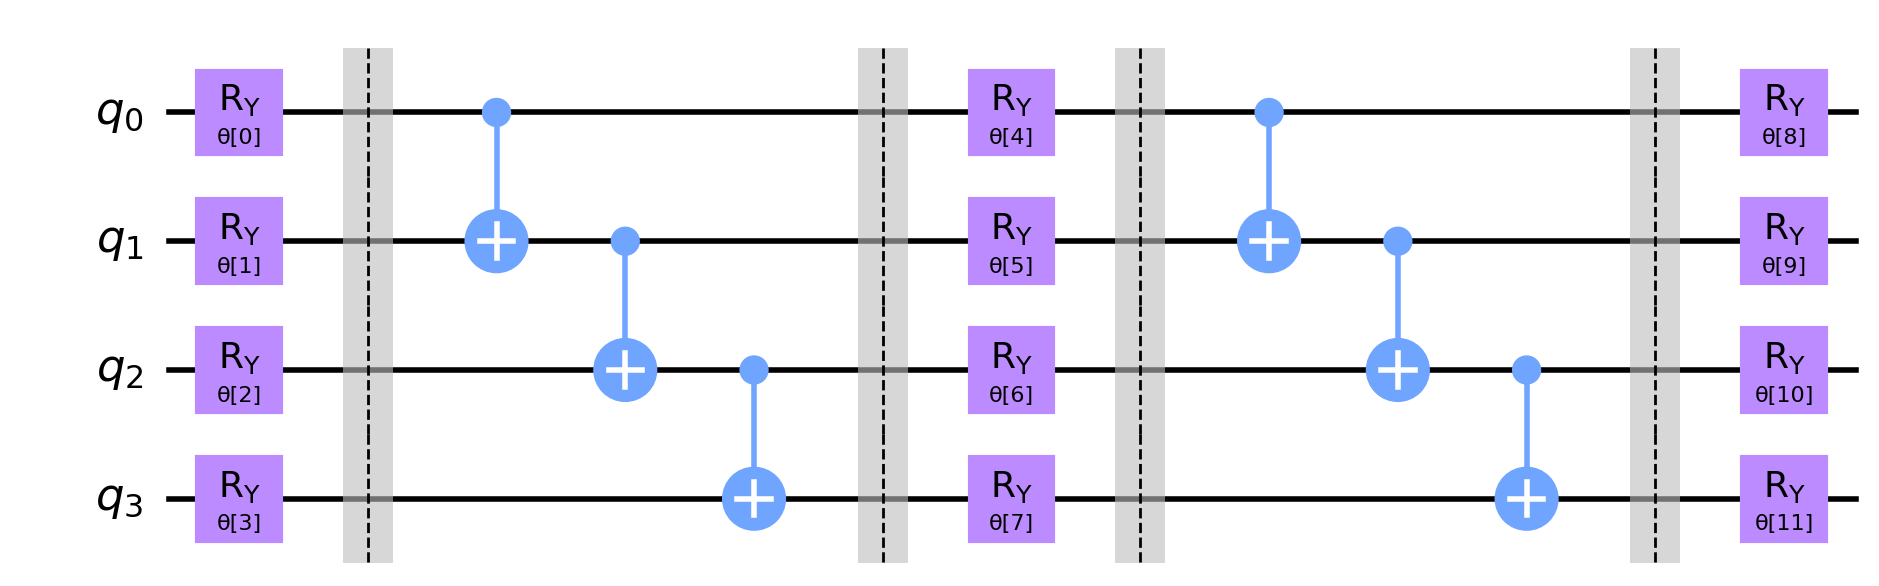
\includegraphics[width=\textwidth]{Artefact/Appendices/ansatz4-2.png}
    \caption{
        Samples of parameterised circuits generated by the Qiskit framework.
        The ansatz is a sequence of rotation layers and entanglement layers.
        Above: an ansatz of three qubits and two repetition layers.
        Below: an ansatz of four qubits and two repetition layers.
    }
    \label{Ansatz samples}
\end{figure}

\subsubsection{Visualise the Gradient}
To calculate the gradient variance, we use the parameter shift rule from Eq. \ref{Parameter-shift rules} as implemented in Qiskit Gradient Framework.
The BP phenomena can be verified when the gradient variance with an increased number of qubits and repetition layers.

To visualise the gradient variances, we have plotted a range of random parameters for each ansatz as the initial starting point.
Such randomised parameters are generated 100 times uniformly to calculate the gradients.
We then plot the variance values of the gradients for different numbers of qubits and repetition values for a range of 2 to 9 qubits and repetition.

In short, we use 100 uniformly randomised parameters to scan the gradient, then we calculate the "slope" of the gradient.

\subsubsection{Experiment with Local Cost Function and Shallow Depth}
The two ansatzes are configured such that their depths are fixed, along with a local cost function.
The \textit{Global Cost Function} is the combined output of all qubits. 
On the other hand, the \textit{Local Cost Function} only compares the values of individual qubits or a subset of qubits \cite{cerezoCostFunctionDependent2021}.